\subsubsection{BackEnd}
Mit Beginn der Backend-Entwicklung wurden in erster Linie die Grundstrukturen implementiert, um der \textit{MVVM}-Architektur gerecht zu werden. Dabei lag 
der Fokus bei der Instanziierung der notwendigen Komponenten der \textit{Android Architecture Components}. Nach chronologischer Reihenfolge wurden die Klassen 
erstellt und mit den dazugehörigen Funktionen und Methoden versehen. Angefangen mit der Entity-Klasse zur Beschreibung des Objekts und deren allgemeiner Aufbau, 
dieser bereits in der Konzeption (\ref{chap:Konzeption}) unter dem Datenmodell (\ref{chap:Datenmodell}) festgehalten wurde. Darauffolgend wurde das „Data Object“ 
erstellt, welches die Zugriffe der Datenbankobjekte managed. Abschließend im Bereich der Datenbank ein Room-Layer, um die eigentliche Datenbank zu 
instanziieren und eine Zugriffsschicht auf diese zu implementieren. 
\\ 
Zur Modularisierung und zur Generierung einer Schnittstelle für den Bezug zu mehreren Datenbeziehungspunkten wurde ein Repository erstellt, das eine saubere 
\acs{API} für den Datenzugriff auf den Rest der Anwendung bietet. Um die vorhandenen Klassen zum Datentransfer und zur Persistierung der Daten mit der 
eigentlichen Benutzeroberfläche zu verbinden, wurde ein ViewModel implementiert, welches die Daten zwischen den einzelnen Komponenten teilt und bereitstellt. 
\\ 
\linebreak 
Nach Aufzählung der einzelnen Bestandteile wird auf diese nun genauer eingegangen. 
\\ 
\linebreak
In einer Java-Klasse wird mithilfe der gegebenen Bibliothek „Room“ ein Entity-Objekt erstellt. Hierbei gibt es eine eindeutige Annotation, die die Klasse und 
deren beinhalteten Variablen deklariert. So wird, dem folgend aufgeführten Code-Beispiel (\ref{code:entity}) zu entnehmen, eine Klasse in eine Entity und somit 
in eine Datenbank-Tabelle konvertiert. In dieser Tabelle, definiert als \textit{„object\_table“}, gibt es weitere Variablen, die mit Annotationen versehen sind. 
Damit werden diese gemäß der Anforderungen des Konzepts definiert. Diese Variablen repräsentieren die Attribute des Datenbankschematas und stellen die einzelnen 
Informations- , bzw. -Datenbankspalten dar. Zur Veranschaulichung die Initialisierung der \acs{ID}-Vergabe eines Objekts. Diese wird als \textit{„id“}-Spalte 
und ebenso als Primärschlüssel\footnote{Einmaliger und eindeutiger Wert einer Tabelle, bzw. eines Attributs, um dieses eindeutig zu kennzeichnen.}-Variable 
deklariert.
\\ 
\linebreak
\begin{lstlisting}[language=C,
    frame=lines,           % Ein Rahmen um den Code (single for box, lines for top and bottom)
    xleftmargin=\parindent,  % Rahmen link von den Zahlen
    style=algoBericht,
    label={code:entity},
    captionpos=b,           % Caption unter den Code setzen
caption={Entity Code zur Initialisierung der Objekte}]
@Entity(tableName = "object_table")
public class Object {
    @ColumnInfo(name = "id")
    @NonNull
    @PrimaryKey(autoGenerate = true)
    private int id;

    public int getId() { return this.id; }
    public void setId(int id) { this.id = id; }
    ... 
}
\end{lstlisting}
\pagebreak
Das mit der Entity-klasse kommunizierende Modul ist das \textit{„Data Object“}, welches als Interface angelegt wurde. Das „Object Dao“ verwendet ebenso die Bibliothek 
„Room“ und wandelt die Java-Klasse per Annotation in ein „Dao“ um, dieses beinhaltet hauptsächlich die SQL-Queries zur Datenabfrage der vorhandenen Informationen. 
\\
\linebreak
\begin{lstlisting}[language=C,
    frame=lines,           % Ein Rahmen um den Code (single for box, lines for top and bottom)
    xleftmargin=\parindent,  % Rahmen link von den Zahlen
    style=algoBericht,
    label={code:query},
    captionpos=b,           % Caption unter den Code setzen
caption={SQL-Query zur Abfrage der Objekt-Namen}]
@Query("SELECT * FROM object_table ORDER BY name")
LiveData<List<Object>> getObjectName();
\end{lstlisting}
Anschließend nachdem die beiden Klassen erstellt waren, wurde das Datenbank-Layer auf der eigentlichen Datenbank implementiert. Über einen „Builder“ wird die 
Datenbank-Instanz erzeugt und mit einem Namen versehen. Im Fall des Assistenzsystems als \textit{„object\_database“} deklariert. 
\\ 
In zukünftiger Entwicklungen, 
falls notwendig, gäbe es die Möglichkeit in diesem Schema weitere Datenbanken zu erstellen und diese über weitere „Dao“s zu referenzieren. Darüber hinaus ist die 
Möglichkeit gegeben weitere Datenbank-Tabellen zu erstellen, um weitere Objekte und Informationen speichern zu können. Ebenso ist durch ein Repository die Option 
geboten, die derzeit auf dem Smartphone gespeicherte Datenbank auf einen externen Server auszulagern, um so die Daten weitläufiger zur Verfügung zu haben. 
Eine Datenbeziehung von generierten Daten der Maschinen und Geräte selbst wäre unter anderem auch vorstellbar, allerdings müssten diese vorab noch aufbereitet 
und zur Nutzung bereitgestellt werden. Diese Methode wird allerdings nicht näher betrachtet, da diese nicht teil dieser Arbeit ist. 
\\ 
Im Ausblick (\ref{chap:Ausblick}) wird darauf nochmals eingegangen.
\\ 
\linebreak
\begin{lstlisting}[language=C,
    frame=lines,           % Ein Rahmen um den Code (single for box, lines for top and bottom)
    xleftmargin=\parindent,  % Rahmen link von den Zahlen
    style=algoBericht,
    label={code:dblayer},
    captionpos=b,           % Caption unter den Code setzen
caption={Erzeugung des Datenbank-Layers „Room“}]
@Database(entities = {Object.class}, version = 1, exportSchema = false)
public abstract class ObjectRoomDatabase extends RoomDatabase {
    ...
    INSTANCE = Room.databaseBuilder(context.getApplicationContext(),
    ObjectRoomDatabase.class, "object_database")
    .addCallback(sRoomDatabaseCallback)
    .build();
    ...
}
\end{lstlisting}
Letzter wichtiger zu implementierender Aspekt war das Kommunikations-Modul zwischen den Datenbank-Transfers und der Benutzeroberfläche, das ViewModel. 
In dieser Klasse wird eine Liste erstellt, welche den Wert des zu speichernden Objekts besitzt. Diese werden über eine „get“-Funktion aus dem zuvor 
instanziierten Repository geladen und in der erzeugten Liste lokal abgelegt. Diese Liste wird dann für die Präsentation der Informationen auf der 
Nutzeroberfläche verwendet. 
\\ 
\linebreak
Ursprünglich war die Implementierung der eigentlichen Scan-Phase unter Beachtung der ARCore-\acs{API} einfach angedacht, die sich im Laufe der Entwicklung 
allerdings als nicht so praktikabel herauskristallisierte. Diese aufgetretene Problemstellung wird in weiterem Verlauf präzisiert, nachdem der eigentliche 
Verlauf geschildert wurde. 
\\ 
Das Fragment auf dem \acl{UI} der Scan-Phase (\ref{pic:scan}) wird als \acs{AR}-Fragment, unter der Benutzung des Sceneform \acs{SDK}s, deklariert. Basierend auf 
dieser Initialisierung können die Interaktionen mit den ARCore-, bzw. Sceneform- Elementen gewährleistet werden. Dadurch ist ebenso die Nutzung der Kamera 
gegeben. Diese Funktionen sind Bestandteile der ARCore- und Sceneform-\acs{API}. Über einen \textit{„FragmentManager“} wird die „.xml“-Datei mit dem darin 
enthaltenen Fragment der ID \textit{„sceneform\_fragment“} initialisiert.
\\
\begin{lstlisting}[language=C,
    frame=lines,           % Ein Rahmen um den Code (single for box, lines for top and bottom)
    xleftmargin=\parindent,  % Rahmen link von den Zahlen
    style=algoBericht,
    label={code:arfragment},
    captionpos=b,           % Caption unter den Code setzen
caption={Initialisierung des Fragments}]
private ArFragment fragment;
...
fragment = (ArFragment)
getSupportFragmentManager().findFragmentById(R.id.sceneform_fragment);
...
\end{lstlisting}
Um anschließend Objekte auf diesem Fragment einblenden zu können, ist es vorab notwendig eine \textit{„Session“} zu generieren, die unter anderem für die 
Konfigurationen der Kamera zuständig ist. Dadurch wird bei Start der Scan-Phase ein dreidimensionales Koordinatensystem erstellt, welches den Ursprungspunkt der 
Anwendung darstellt. Mit Verwendung der internen Sensoren des Smartphones werden darauffolgende Bewegungen registriert und mittels \acs{SLAM} Verfahren berechnet. 
So ist die Kalkulation der Lokalisation möglich und anhand der Kamera kann auf Basis des \acs{SLAM} Verfahrens die Umgebung abgebildet werden. Durch diese 
Gegebenheiten wird die virtuelle Karte des Umfelds erzeugt und dient so zur Veranschaulichung der zu platzierenden Objekte. In der Abbildung (\ref{pic:koordin}) 
ist ein Beispiel zu sehen, indem ein Objekte erstellt wird, welches die Koordinaten von dem Ursprungspunkt berechnet. So wird deutlich, wie die Position eines 
Objekts errechnet wird, unter der Verwendung des von ARCore gegebenen \acs{SLAM} Verfahrens. Vorausgesetzt der Anwender startet an der Position (x,y,z = 0), 
bewegt sich frei im Raum und setzt an Postion (x = 5, y = 1, z = 3.5) ein Objekte.
\begin{figure}[hbt!]
    \centering
    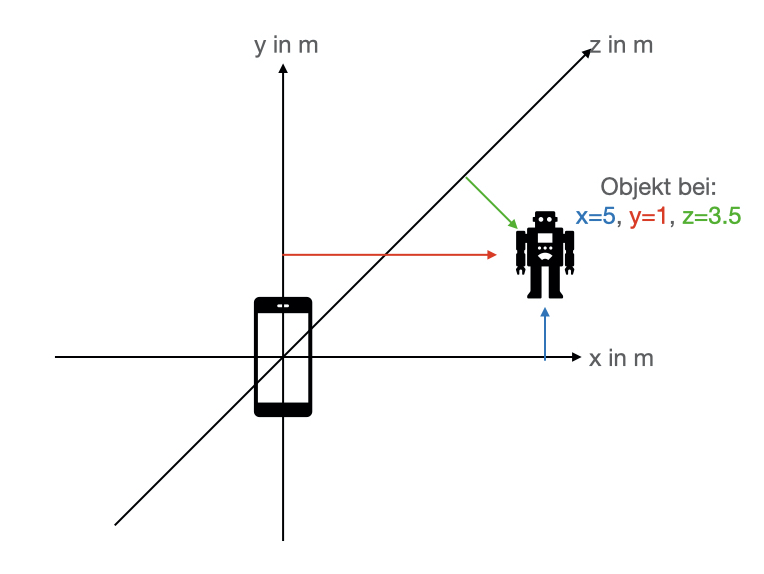
\includegraphics[width=10cm,height=10cm,keepaspectratio]{4Umsetzung/Bilder/koordin.jpeg}
    \caption{Aufbau der Positionsberechnung von Objekten}
    \label{pic:koordin}
\end{figure}
\\ 
Beim setzen eines Objekts wird als Anhaltspunkt der Mittelpunkt des Bildschirms berechnet, um das Objekt zentriert platzieren zu können. Ist 
diese Position berechnet, ist durch Hilfe des \acs{SLAM} Verfahrens die genaue virtuelle Position zu ermitteln und anhand dieser ist das Objekt 
zu platzieren. 
\\ 
Das Objekte wird gesetzt, indem der Nutzer in der \acs{UI} (\ref{pic:scan}) im Bereich der „Gallery“ ein Objekt anklickt.
Über die der Sceneform-\acs{API} zur Verfügung gestellte Methode („ModelRenderable“) wird das Objekt erstellt und als „Anchor“ auf die berechnete Position 
gesetzt. Ein Anchor ist die fixe Position des Objekts, an dem dies platziert wird und so lange dort vorhanden bleibt, bis die Applikation beendet wird. Die Datei 
die als dreidimensionales asset genereirt werden soll, wird über die „uri“-Variable übergeben. 
\begin{lstlisting}[language=C,
    frame=lines,           % Ein Rahmen um den Code (single for box, lines for top and bottom)
    xleftmargin=\parindent,  % Rahmen link von den Zahlen
    style=algoBericht,
    label={code:modelrenderable},
    captionpos=b,           % Caption unter den Code setzen
caption={ModelRenderable Builder}]
ModelRenderable.builder()
.setSource(owner.get(), uri)
.build()
.handle((renderable, throwable) -> {
    ...
}
\end{lstlisting}
Während der Objekt-Renderung öffnet sich die \acs{GUI} (\ref{pic:createObject}) zur Eingabe der Informationen, die sich auf das Objekt beziehen. Diese 
werden dann zusammen mit der virtuellen Position des Objekts abgegriffen und in die Datenbank geschrieben. Drückt der Anwender den „save“-Button der Oberfläche 
beendet er diesen Vorgang und kehrt auf die \acs{UI} der Scan-Phase zurück, um weiter Objekte platzieren zu können. 
\\ 
Zu der Position des Objekts wird dessen Rotation durch die einfache Berechnung durch Quaternionen ebenso in die Datenbank gespeichert, um die Darstellung so real 
wie möglich wiederzugeben. Damit erfolgt die Feststellung, dass das Objekt immer in Blickrichtung der Kamera positioniert ist, da die Rotation ausgehen von der 
Kamerahaltung berechnet wird. 
%--> Problemschilderung der Speicherung der Session
\\ 
\linebreak
Ursprünglich war geplant, die generierte Session sowie die darin erstellten Objekte in der Datenbank abzuspeichern, um diese bei erneutem Aufruf der 
Scan-Phase, bzw. bei Anwendung der Visualisierungs-Phase zu laden und innerhalb dieser Session wieder anzeigen zu lassen. Da die Datenbank nur gewisse Datentypen 
zulässt, war das erste auftretende Problem die Speicherung der Session als Objekt, welches zunächst in eine „BLOB“-Datei konvertiert wurde, um diese speichern 
zu können. Eine „BLOB“-Datei ist ein Binary Large Object, welches anhand der Binärcodierung abgespeichert wird. Dabei kann es sich unter anderm um große 
Bild- oder Audio-Dateien handeln, auch können so anderweitig große Dateien gespeichert werden. Mit dieser Umsetzung tat sich auch schon das nächste Problem auf, 
welches deutlich schwerwiegender war und auch in diesem Sinne die Visualisierungs-Phase betraf. 
\\ 
Da eine erzeugte Session nur eine gewissen Zeit verwendet wird, ist diese für den weitern Gebrauch nicht vorgesehen, dies bedeutet, dass nach erneutem Starten 
des Assistenzsystems alle zuvor erzeugten Objekte zwar auf die dazugehörige Session bestimmt sind, allerdings auf der zugewiesenen Position 
nicht mehr erreichbar wären. Durch die Unterschiedlichen Startpunkte, die bei wiederholtem Starten der Anwendung erzeugt worden würden, 
würde sich die ursprüngliche Ausgangsposition der Applikation verschieben und so auch die Objekte an eine fälschliche Position projizieren. Somit wäre das 
Ergebnis nicht exakt und könnte keine Anwendung finden, da die Applikation Informationen anzeigen würde, die der Realität nicht entsprechen. 
\\ 
Basierend auf dieser Erkenntnis musste umdisponiert und ein neuer Lösungsansatz konzipiert werden. Mit dem Wissen über den aktuellen Stand der ARCore \acs{API} 
war es die neue Aufgabe eine Lösung zu entwickeln, welche exakt und zuverlässig arbeitet, um Informationen nicht inkorrekt zu interpretieren. 
\\ 
Dieser Ansatz wird nun erläutert.
\\ 
\linebreak
Die Idee war es, einen Fixpunkt zu erstellen, welcher dazu diente einen immer gleichbleibenden Startpunkt vorzugeben. Dadurch gäbe es keine Unterschiede des 
Ausgangspunktes mehr und der Nutzer könnte trotz seiner aktuellen Position starten. Dazu muss er beim Start der Applikation an den Ursprungspunkt kehren, 
um daraufhin die Funktion zu starten. Für diesen Ansatz wurde ein Marker gewählt (siehe Abbildung \ref{pic:initialMarker}), der vor dem ersten Gebrauch 
der Software an einer Position angebracht wird und an dieser dauerhaft bestehen bleibt. 
\begin{figure}[hbt!]
    \centering
    
\includegraphics[width=5cm,height=5cm,keepaspectratio]{4Umsetzung/Bilder/cjt_logo_tracking.png}
    \caption{Marker zur Erkennung der Ausgangsposition}
    \label{pic:initialMarker}
\end{figure}
\\
Um diesen Ansatz umsetzen zu können, war es notwendig eine weitere Funktion zur Applikation hinzuzufügen (siehe Abbildung \ref{pic:image_tracking} 
in Scan-Phase \ref{chap:scan_implementation} Frontend), damit ein Marker verfolgt werden kann. Wird dieser Marker erkannt, folgt die eigentliche Scan-Phase, 
die nach der Umkonzeptionierung sowohl bei der Objektplatzierung als auch bei der Datenspeicherung ebenso überarbeitet wurde. 
\\ 
\linebreak
Angenommen der Nutzer starten die Applikation an einer beliebigen Position im Raum und platziert Objekte an von ihm vorgesehenen Stellen, dann wurden die 
Objekte erstellt, aber keinerlei Anhaltspunkte geschaffen, um bei nachzutragenden Objekten die gleichen Voraussetzungen zu erfüllen. Daher wird bei der Scan-Phase 
die Methode zur Markererkennung eingebaut, um einen initialen Fixpunkt zu erstellen. Dadurch ist es gewährleistet, ausgehend von diesem Punkt erneut Objekte zu 
platzieren, egal wo im Raum die Applikation gestartet wurde. Da die Objekte immer zu so erstellt werden, dass sie abhängig zur Position des Fixpunktes gespeichert 
und angezeigt werden. Dies bedeutet, die Objekte sind immer eine Referenz zu dem initialen Marker. Auch wenn ein Objekt nachträglich hinzugefügt werden soll, ist 
es lediglich vom Nutzer erforderlich den Marker einzuscannen und danach an die gewünschte Position, an der das Objekt platziert werden soll, zu laufen und das 
Objekt erstellen. Demnach wird auch beim Schreibbefehl, in die Datenbank, lediglich die Differenz, bzw. der Abstand zu dem initialen Marker gespeichert, um immerzu 
diese Position als Ursprungspunkt zu nehmen. Die Berechnung der Distanz zwischen Objekt und Ursprungsmarker erfolgt durch eine präzise Subtraktion, bei der 
lediglich die Ursprungskoordinaten von den aktuellen Positionskoordinaten subtrahiert werden. Dieser Vorgang ist dem folgenden Code-Beispiel (\ref{chap:AAC}) zu 
entnehmen. Dabei wird das aktuelle Objekt „object“ und das initiale Objekt „initialObject“ als Parameter übergeben, die sogenannte „call by Reference“, um die 
Distanz berechnen zu können. Das Ergebnis wird in mehreren lokalen Variablen zwischengespeichert und zum Schluss in eine neue Position „Pose“ mit Position und 
Rotation, von der Berechnung durch Quaternionen, ermittelt. Der Rückgabewerte diese Funktion ist demnach eine „Pose“, die nach Aufruf der Methode übergeben 
und so in der Datenbank hinterlegt wird. Mit dem Resultat ist demnach die Position und Rotation des einzelnen Objekts gegeben und kann in der Visualisierungs-Phase 
verwendet werden.
\begin{lstlisting}[language=C,
    frame=lines,           % Ein Rahmen um den Code (single for box, lines for top and bottom)
    xleftmargin=\parindent,  % Rahmen link von den Zahlen
    style=algoBericht,
    label={code:differencetoinitial},
    captionpos=b,           % Caption unter den Code setzen
caption={Berechnung der Distanz zwischen Marker und Ursprungspunkt}]
public Pose returnValueFromPosition(Object object, Object initialObject){
    float tX = object.getTx() - initialObject.getTx();
    float tY = object.getTy() - initialObject.getTy();
    float tZ = object.getTz() - initialObject.getTz();

    float qX = object.getQx() - initialObject.getQx();
    float qY = object.getQy() - initialObject.getQy();
    float qZ = object.getQz() - initialObject.getQz();
    float qW = object.getQw() - initialObject.getQw();

    float[] rotation = {qX,qY,qZ,qW};
    float[] translation = {tX,tY,tZ};

    return new Pose(translation, rotation);
}
\end{lstlisting}
Zur Veranschaulichung der zuvor beschriebenen Methodik dient die Abbildung (\ref{pic:differenztoinitial}). Durch diese Skizze wird nochmals verdeutlicht, dass 
sich alles in einem erstellten Koordinatensystem abspielt und lediglich die Distanz der einzelnen Objekte zum Marker berechnet und in der Datenbank persistiert 
werden.
\begin{figure}[hbt!]
    \centering
    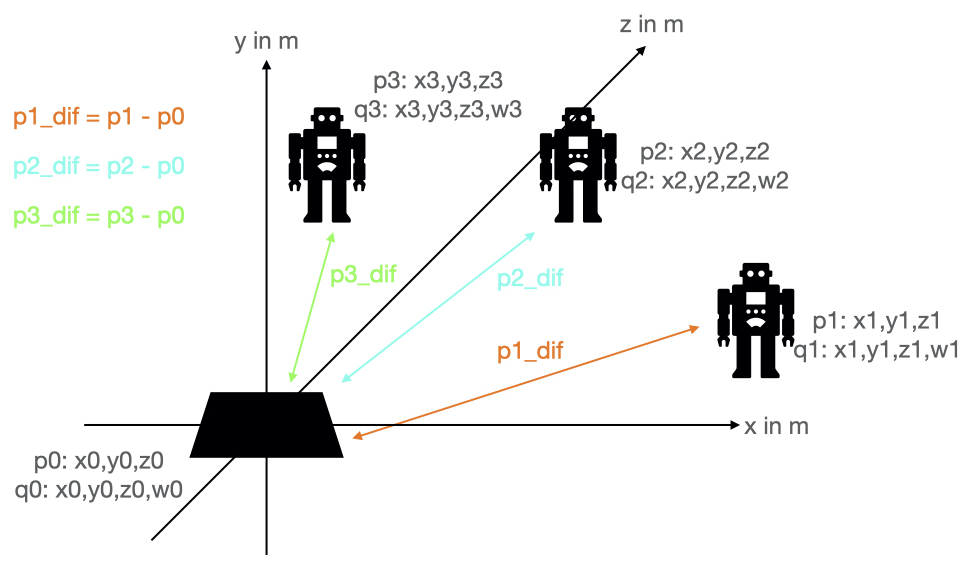
\includegraphics[width=14cm,height=14cm,keepaspectratio]{4Umsetzung/Bilder/difcalc.jpeg}
    \caption{Positionsberechnung zum Ursprungsmarker}
    \label{pic:differenztoinitial}
\end{figure}
\\ 
Nachdem die Scan-Phase nun vollends beschrieben wurde, geht es in folgendem Kapitel um die Erläuterung des dritten und letzten Use Cases. Dabei werden sowohl 
die Frontend als auch die Backend Aspekte aufgezeigt. 